

\chapter{Sistema de informação: análise de requisitos e arquitetura}




\section{Modulação}

\subsection{Análise de requisitos}


\subsubsection{Entidades envolventes}


\subsection{Casos de uso}





\section{Diagramas}


\subsection{Entidade-relação}









\begin{table}[h]
	\centering
	
	\begin{tabular}{|
			>{\columncolor[HTML]{EFEFEF}}l |l|}
		\hline
		\textbf{Caso de utilização:} & \begin{tabular}[c]{@{}l@{}}-dasdasdasasdasdddddddddddddddddddddddd\\ -dasdasd\\ -dasdasda\end{tabular} \\ \hline
		\textbf{Ator:} &  \\ \hline
		\textbf{Descrição:} &  \\ \hline
		\textbf{Pré-condições:} &  \\ \hline
		\textbf{Pós-condições:} &  \\ \hline
	\end{tabular}
	\caption{Casos de utilização: Login/Logout}
	\label{my-label}
\end{table}




\subsection{Modelo relacional}


\subsection{Estrutura final}


\newpage

\section{Requisitos de funcionamento}



\section{Tecnologias de desenvolvimento}



\subsection{Base de dados}



\section{Sistema de gestão de base de dados}


\subsection{PostgreSQL}


\subsection{SQL server}



\subsection{Solução adoptada}




\subsection{\textit{Web}}




\section{Frameworks de desenvolvimento web}


Manipulação local usando JS do DOM
Angular, React

Servidor serve conteudos criados em função dos pedidos do cliente 




\subsection{\textit{Mobile}}

\section{Frameworks/tecnologias de desenvolvimento mobile}



\subsection{Android nativo}

\subsection{Ios nativo}

\subsection{Multi-plataforma}

http://websocialdev.com/lista-de-frameworks-para-desenvolvimento-mobile/




\section{Casos de utilização}

\begin{figure}[!htb]
	\centering
	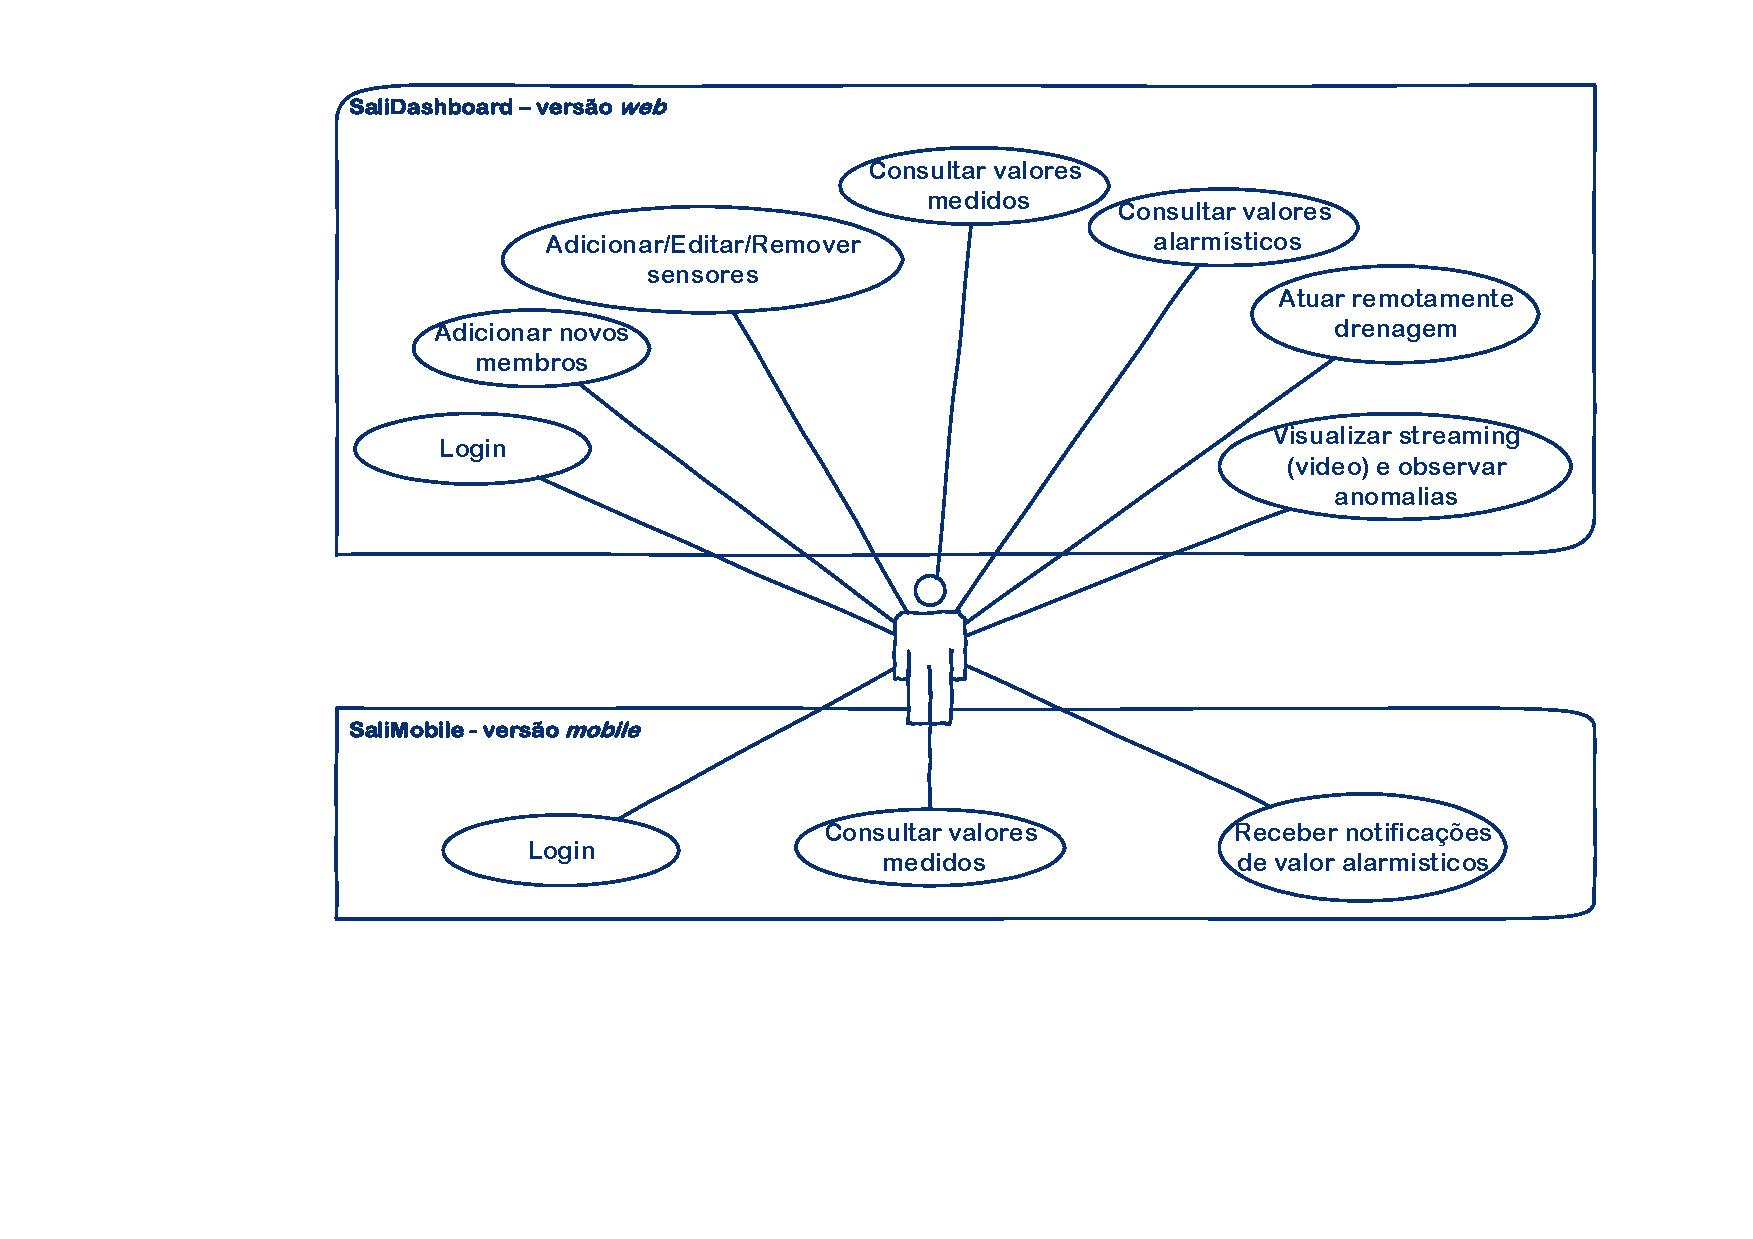
\includegraphics[scale=0.5]{esquemas/usecases.pdf}
	\caption{Pirâmide do conhecimento: modelo DIKW}
	\label{dikw}
\end{figure}



\section{API rest}

com autenticação via token 

\subsection{Documentação API}

utilizado swagger; apenas permite acesso a quem está logado... incorporar layout do swagger com o do salidashboard




app mobile
microcontroladores -> controller modulers 


documentação com swager 





\section{Simulação da API}

\section{Valores simulados}



\section{\textit{Deploy} do projecto}


https://jee-appy.blogspot.com.tr/2015/04/deploy-django-project-on-apache-using.html

Caracteristicas da maquina virtual

Description:	Ubuntu 14.04.1 LTS
64 bitsRAM 2GB 

\section{Considerações finais}








